% latex uft-8
\documentclass[uplatex,dvipdfmx,a4paper,11pt,oneside,openany]{jsbook}
%
\usepackage[dvipdfmx]{graphicx}
\usepackage{amsmath,amssymb}
\usepackage{bm}
\usepackage{physics}
\usepackage{graphicx}
\usepackage{ascmac}
\usepackage{amsmath}
\usepackage{setspace}
\usepackage{here}
\usepackage{fancybox}
\usepackage{url}
\usepackage{listings,jlisting} %日本語のコメントアウトをする場合jlistingが必要
\usepackage{xcolor}
\usepackage{comment}
\usepackage{multicol}
\usepackage{amsmath, amssymb}
\usepackage{type1cm}
\usepackage{booktabs}
\usepackage{multirow}

\definecolor{mygreen}{rgb}{0,0.6,0}
\definecolor{mygray}{rgb}{0.5,0.5,0.5}
\definecolor{mymauve}{rgb}{0.58,0,0.82}

%\begin{comment}
\lstset{
  backgroundcolor=\color{white},   % choose the background color; you must add \usepackage{color} or \usepackage{xcolor}; should come as last argument
  basicstyle=\footnotesize,        % the size of the fonts that are used for the code
  breakatwhitespace=false,         % sets if automatic breaks should only happen at whitespace
  breaklines=true,                 % sets automatic line breaking
  captionpos=b,                    % sets the caption-position to bottom
  commentstyle=\color{mygreen},    % comment style
  deletekeywords={...},            % if you want to delete keywords from the given language
  escapeinside={\%*}{*)},          % if you want to add LaTeX within your code
  extendedchars=true,              % lets you use non-ASCII characters; for 8-bits encodings only, does not work with UTF-8
  firstnumber=1000,                % start line enumeration with line 1000
  frame=single,	                   % adds a frame around the code
  keepspaces=true,                 % keeps spaces in text, useful for keeping indentation of code (possibly needs columns=flexible)
  keywordstyle=\color{blue},       % keyword style
  language=Octave,                 % the language of the code
  morekeywords={*,...},            % if you want to add more keywords to the set
  numbers=left,                    % where to put the line-numbers; possible values are (none, left, right)
  numbersep=5pt,                   % how far the line-numbers are from the code
  numberstyle=\tiny\color{mygray}, % the style that is used for the line-numbers
  rulecolor=\color{black},         % if not set, the frame-color may be changed on line-breaks within not-black text (e.g. comments (green here))
  showspaces=false,                % show spaces everywhere adding particular underscores; it overrides 'showstringspaces'
  showstringspaces=false,          % underline spaces within strings only
  showtabs=false,                  % show tabs within strings adding particular underscores
  stepnumber=2,                    % the step between two line-numbers. If it's 1, each line will be numbered
  stringstyle=\color{mymauve},     % string literal style
  tabsize=2,	                   % sets default tabsize to 2 spaces
  title=\lstname                   % show the filename of files included with \lstinputlisting; also try caption instead of title
}
%\end{comment}

\lstdefinelanguage{mypy}{
  % リテラルと演算記号
  morekeywords=[1]{+=,=,==,!=,!,>,<,>=,<=,++,-,+,*,\%,/},
  % 予約語
  morekeywords=[2]{False,None,True,and,as,assert,async,await,break,
    class,continue,def,del,elif,else,except,finally,for,from,global,
    if,import,in,is,lambda,nonlocal,not,or,pass,raise,return,try,while,
    with,yield,print,match,case
  },
  % 識別子
  morekeywords=[3]{defined_func},
  % 区切り文字を強制的に色付け
  literate=*{.}{{\color{delimiter}.}}1
            {,}{{\color{delimiter},}}1 {:}{{\color{delimiter}:}}1
            {)}{{\color{delimiter})}}1 {(}{{\color{delimiter}(}}1
            {[}{{\color{delimiter}[}}1 {]}{{\color{delimiter}]}}1
            {\{}{{\color{delimiter}\{}}1 {\}}{{\color{delimiter}\}}}1,
  % 大文字小文字を区別
  sensitive=true,
  % 行コメントの設定
  morecomment=[l]{\#},
  % Stringリテラルの設定
  morestring=[b]{\'},
  morestring=[b]{\"},
  % 単語として扱う文字
  alsoletter={\%<>=+-*\/1234567890!},
  % 枠
  frame=none,
  % 長くなったら途中で改行
  breaklines=true,
  % 自動改行時のインデント
  breakindent=12pt,
  % 文字間隔を一定に
  columns=fixed,
  % 文字の横のサイズを小さく
  basewidth=0.5em,
  % 行番号を左に
  numbers=left,
  % 行番号の書式
  numberstyle={\scriptsize\color{white}},
  % 行番号の増加数は1=連番に
  stepnumber=1,
  % フレームの左の余白
  framexleftmargin=18pt,
  % スペースを省略せず保持
  keepspaces=true,
  % インデントサイズ
  tabsize=4,
  backgroundcolor={},                                   % 背景色=透明
  basicstyle={\small\ttfamily\color{white}},            % 通常部分の書式
  identifierstyle={\small\color{white}},                % 識別子の書式
  commentstyle={\small\color{comment}},                 % コメントの書式
  keywordstyle=[1]{\small\bfseries\color{literal}},     % リテラルと演算記号の書式
  keywordstyle=[2]{\small\bfseries\color{reserved}},    % 予約語の書式
  keywordstyle=[3]{\small\bfseries\color{identifier}},  % 自分で定義した識別子の書式
  stringstyle={\small\ttfamily\color{literal}},         % 文字列の書式
}
%ここからソースコードの表示に関する設定
\lstdefinestyle{customc}{
  belowcaptionskip=1\baselineskip,
  breaklines=true,
  numbers=left,
  frame=single,
  xleftmargin=\parindent,
  language=C,
  showstringspaces=false,
  basicstyle=\footnotesize\ttfamily,
  keywordstyle=\bfseries\color{green!40!black},
  commentstyle=\itshape\color{purple!40!black},
  identifierstyle=\color{blue},
  stringstyle=\color{orange},
}

\lstdefinestyle{custompy}{
  belowcaptionskip=1\baselineskip,
  breaklines=true,
  numbers=none,
  frame=l,
  xleftmargin=\parindent,
  language=python,
  showstringspaces=false,
  basicstyle=\footnotesize\ttfamily,
  keywordstyle=\bfseries\color{green!40!black},
  commentstyle=\itshape\color{purple!40!black},
  identifierstyle=\color{blue},
  stringstyle=\color{orange},
}

\lstdefinestyle{customasm}{
  belowcaptionskip=1\baselineskip,
  frame=L,
  xleftmargin=\parindent,
  language=[x86masm]Assembler,
  basicstyle=\footnotesize\ttfamily,
  commentstyle=\itshape\color{purple!40!black},
}

\lstset{escapechar=@,style=custompy}
\renewcommand{\lstlistingname}{プログラム}

\begin{comment}
\makeatletter
\def\ps@plainfoot{%
  \let\@mkboth\@gobbletwo
  \let\@oddhead\@empty
  \def\@oddfoot{\normalfont\hfil-- \thepage\ --\hfil}%
  \let\@evenhead\@empty
  \let\@evenfoot\@oddfoot}
  \let\ps@plain\ps@plainfoot
  \renewcommand{\chapter}{%
  \if@openright\cleardoublepage\else\clearpage\fi
  \global\@topnum\z@
  \secdef\@chapter\@schapter}
\makeatother
\end{comment}

%
\newcommand{\maru}[1]{{\ooalign{%
\hfil\hbox{$\bigcirc$}\hfil\crcr%
\hfil\hbox{#1}\hfil}}}
%
\setlength{\textwidth}{\fullwidth}
\setlength{\textheight}{40\baselineskip}
\addtolength{\textheight}{\topskip}
\setlength{\voffset}{-0.55in}
%
\makeatletter
\newenvironment{tablehere}
  {\def\@captype{table}}
  {}
\newenvironment{figurehere}
  {\def\@captype{figure}}
  {}
\makeatother
%
\title{魔方陣}
\author{smat1957@gmail.com\thanks{https://altema.is.tohoku.ac.jp/QA4U3/}}
\date{\today}
%
\begin{document}

\maketitle

\chapter{魔方陣を量子アニーリングで解く}

魔方陣は、$N\times N$の各セルに$1\sim N^2$の数値を一つずつ入れ、縦横斜めのどの列についても、その列の数値の総和が等しくなる様に、数値を配置するもの。

例えば$3\times 3$の魔方陣であれば、縦横斜めのどの列にある数値の総和も等しく$15$になる。

\begin{figure}[htbp]
  \begin{center}
  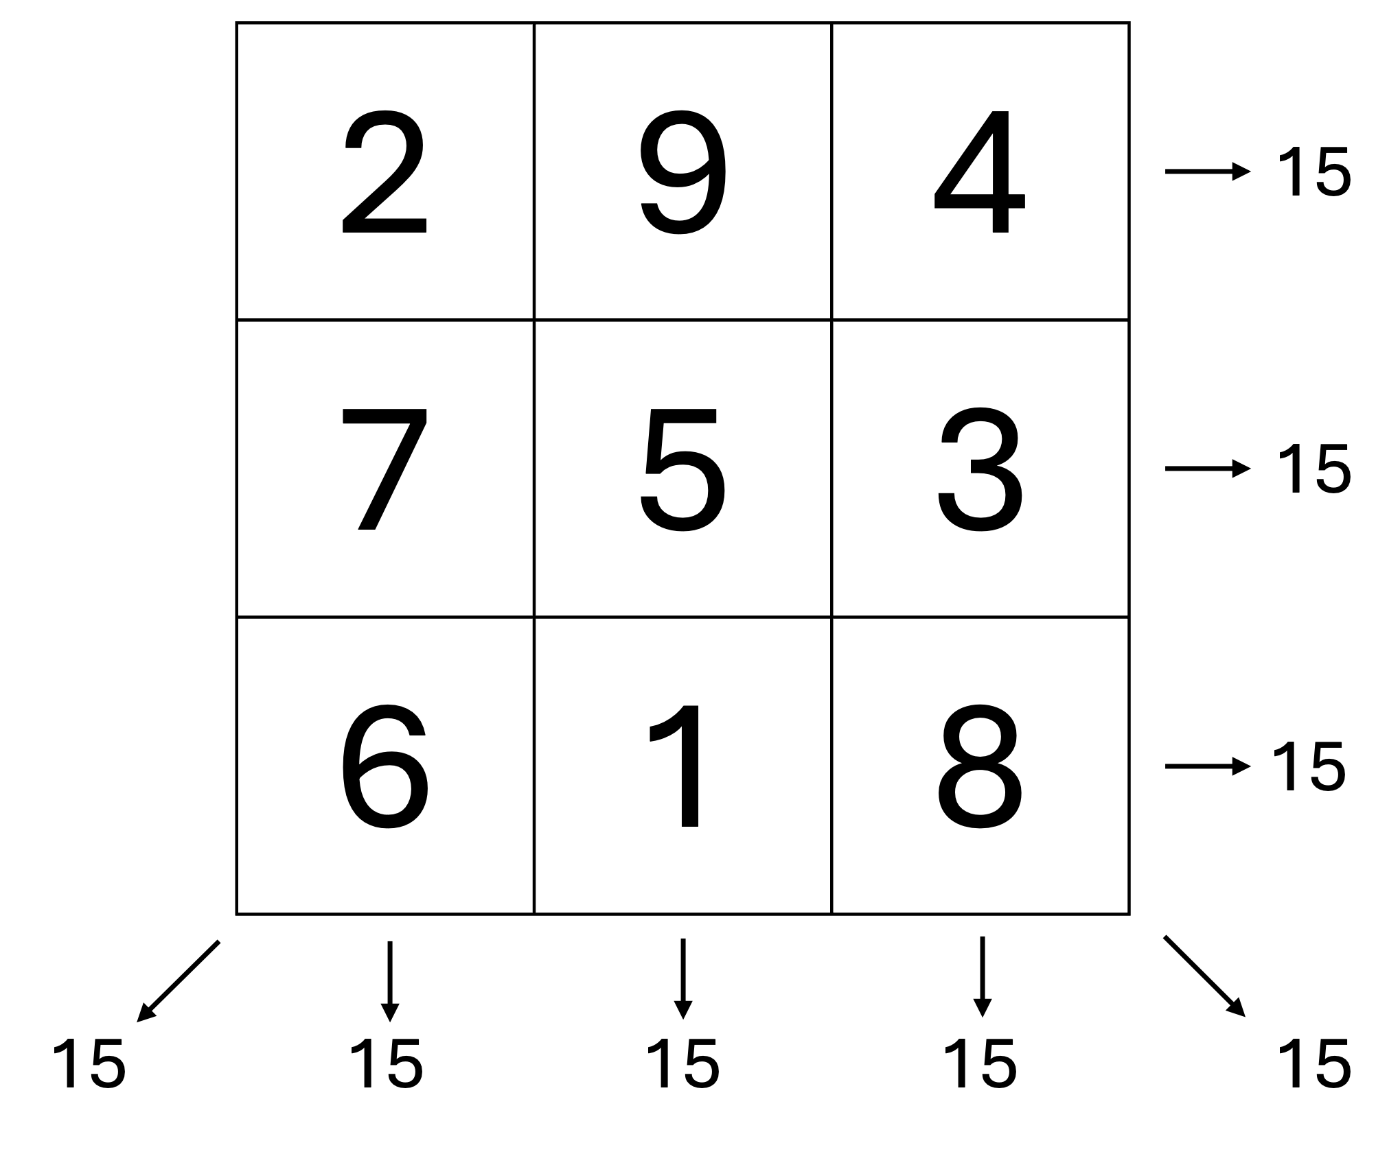
\includegraphics[width=40mm]{f1.png}
  \caption{参考資料\cite{b2}より}
  \end{center}
\end{figure}

$3\times3$は、対称な形を1つと数えることにすると1通り、$4\times4$では880通り、$5\times5$では275305224通り、$6\times6$では17753889197660635632通り存在することがわかっている。\cite{b2}

\section{問題の構成}

決定変数$q$を各セル毎に$N\times N$個用意する。$q_{i,j,n}$は、$i$行$j$列目のセル内の$N\times N$個の決定変数。\\ここで、$i, j\;\in\{1, 2, \cdots, N\},\;n\;\in\{1, 2, \cdots, N\times N\}$。表は$N=3$の場合。

\begin{center}
\begin{tabular}{|c||c|c| c |c||c|c| c |c||c|c| c |c|} \hline
  &\multicolumn{4}{|c||}{1列目($j=1$)}&\multicolumn{4}{|c||}{2列目($j=2$)}&\multicolumn{4}{|c|}{3列目($j=3$)}\\\hline\hline
  \multirow{2}{*}{1行目}&\multicolumn{4}{|c||}{セル($i=1, j=1$)}&\multicolumn{4}{|c||}{セル($i=1, j=2$)}&\multicolumn{4}{|c|}{セル($i=1, j=3$)}\\\cline{2-13}
  &1&2& $\cdots$ &9& 1&2& $\cdots$ &9& 1&2&$\cdots$ &9 \\\cline{2-13}
  ($i=1$)&$q_{111}$&$q_{112}$& $\cdots$ &$q_{119}$& $q_{121}$&$q_{122}$&$\cdots$&$q_{129}$& $q_{131}$&$q_{132}$&$\cdots$&$q_{139}$ \\\hline\hline
  %& & & $\cdots$ & & &  & &$\cdots$& &  & & & $\cdots$ & & \\\hline\hline
  \multirow{2}{*}{2行目}&\multicolumn{4}{|c||}{セル($i=2, j=1$)}&\multicolumn{4}{|c||}{セル($i=2, j=2$)}&\multicolumn{4}{|c|}{セル($i=2, j=3$)}\\\cline{2-13}
  &1&2& $\cdots$ &9& 1&2& $\cdots$ &9& 1&2&$\cdots$ &9 \\\cline{2-13}
  ($i=2$)&$q_{211}$&$q_{212}$& $\cdots$ &$q_{219}$& $q_{221}$&$q_{222}$&$\cdots$&$q_{229}$& $q_{231}$&$q_{232}$&$\cdots$&$q_{239}$ \\\hline\hline
  %& & & $\cdots$ & & &  & &$\cdots$& &  & & & $\cdots$ & & \\\hline\hline
  \multirow{2}{*}{3行目}&\multicolumn{4}{|c||}{セル($i=3, j=1$)}&\multicolumn{4}{|c||}{セル($i=3, j=2$)}&\multicolumn{4}{|c|}{セル($i=3, j=3$)}\\\cline{2-13}
  &1&2& $\cdots$ &9& 1&2& $\cdots$ &9& 1&2&$\cdots$ &9 \\\cline{2-13}
  ($i=3$)&$q_{311}$&$q_{312}$& $\cdots$ &$q_{319}$& $q_{321}$&$q_{322}$&$\cdots$&$q_{329}$& $q_{331}$&$q_{332}$&$\cdots$&$q_{339}$ \\\hline
  %& & & $\cdots$  & & &  & &$\cdots$& &  & & & $\cdots$ & & \\\hline
\end{tabular}
\end{center}

この決定変数は0か1かの2値変数で、当該数値$1\sim N\times N$をそのセルに置く(1)か置かない(0)かを表すものとする。
すると制約条件は、次の様に考えることができる。($M=N\times N$とする)

\begin{enumerate}
\item 各セルの中では$1\sim 9$の中のどれか1つだけが1になる(セルに2つ以上の数値は入らない)\\
$\rightarrow \sum_i q_i=1 \; (for\; cell=1\sim 9)$
\begin{equation*}
  f_1 = \sum_i^N\sum_j^N\bigg(\sum_n^M q_{i,j,n} - 1\bigg)^2
\end{equation*}
\item あるセルの数値と同じ数値は、他のセルには入らない\\
$\rightarrow (q_i+q_{i+9}+q_{i+2\times9}+\cdots+q_{i+8\times9})=\sum_{cell=1}^9 q_{i+(cell-1)\times9}=1 \;(for\; i=1\sim9)$
\begin{equation*}
  f_2 = \sum_n^M\bigg(\sum_i^N\sum_j^N q_{i,j,n} - 1\bigg)^2
\end{equation*}
\item いずれの行方向の数値の和も同じ値S($=15$)になる\\
$\rightarrow \sum_{cell=1}^3(\sum_{i=1}^9 i\times q_{i+(cell-1)\times9})=15$ \\
\hspace{12pt}$\sum_{cell=4}^6(\sum_{i=1}^9 i\times q_{i+(cell-1)\times9})=15$ \\
\hspace{12pt}$\sum_{cell=7}^9(\sum_{i=1}^9 i\times q_{i+(cell-1)\times9})=15$
\begin{equation*}
  f_3 = \sum_i^N\bigg(\sum_j^N\sum_n^M n \cdot q_{i,j,n} - S\bigg)^2
\end{equation*}
\item いずれの列方向の数値の和も同じ値S($=15$)になる\\
$\rightarrow \sum_{cell=1,4,7}(\sum_{i=1}^9 i\times q_{i+(cell-1)\times9})=15 $ \\
\hspace{12pt}$\sum_{cell=2,5,8}(\sum_{i=1}^9 i\times q_{i+(cell-1)\times9})=15 $\\
\hspace{12pt}$\sum_{cell=3,6,9}(\sum_{i=1}^9 i\times q_{i+(cell-1)\times9})=15$
\begin{equation*}
  f_4 = \sum_j^N\bigg(\sum_i^N\sum_n^M n \cdot q_{i,j,n} - S\bigg)^2
\end{equation*}
\item 右下がりの対角要素の和と右上がりの対角要素の和も同じ値S($=15$)になる\\
$\rightarrow \sum_{cell=1,5,9}(\sum_{i=1}^9 i\times q_{i+(cell-1)\times9})=15 $\\
\hspace{12pt}$\sum_{cell=3,5,7}(\sum_{i=1}^9 i\times q_{i+(cell-1)\times9})=15$
\begin{equation*}
  f_5 = \bigg(\sum_d^N\sum_n^M n\cdot q_{d,d,n} - S\bigg)^2 + \bigg(\sum_d^N\sum_n^M n \cdot q_{d,N-d+1,n} - S\bigg)^2
\end{equation*}
\end{enumerate}

\begin{comment}
\subsection{式の展開}

\begin{eqnarray*}
  f_1 &=& \sum_i^N\sum_j^N\bigg(\sum_n^M q_{i,j,n} - 1\bigg)^2\\
  &=& \sum_i\sum_j\bigg(\sum_{n_1}\sum_{n_2}q_{i,j,n_1}q_{i,j,n_2} - 2 \sum_n q_{i,j,n}\bigg)\\
  f_2 &=& \sum_n^M\bigg(\sum_i^N\sum_j^N q_{i,j,n} - 1\bigg)^2\\
  &=& \sum_n\bigg(\sum_{i_1}\sum_{j_1}q_{i_1,j_1,n}\sum_{i_2}\sum_{j_2}q_{i_2,j_2,n} - 2 \sum_i\sum_j q_{i,j,n}\bigg)\\
  f_3 &=& \sum_i^N\bigg(\sum_j^N\sum_n^M n \cdot q_{i,j,n} - S\bigg)^2\\
  &=& \sum_i\bigg(\sum_{j_1}\sum_{n_1}n_1\cdot q_{i,j_1,n_1}\sum_{j_2}\sum_{n_2}n_2\cdot q_{i,j_2,n_2} - 2\cdot S\sum_j\sum_n n\cdot q_{i,j,n}\bigg)\\
  f_4 &=& \sum_j^N\bigg(\sum_i^N\sum_n^M n \cdot q_{i,j,n} - S\bigg)^2\\
  &=& \sum_j\bigg(\sum_{i_1}\sum_{n_1}n_1\cdot q_{i_1,j,n_1}\sum_{i_2}\sum_{n_2}n_2\cdot q_{i_2,j,n_2} - 2\cdot S\sum_i\sum_n n\cdot q_{i,j,n}\bigg)\\
  f_5 &=& \bigg(\sum_d^N\sum_n^M n\cdot q_{d,d,n} - S\bigg)^2 + \bigg(\sum_d^N\sum_n^M n \cdot q_{d,N-d+1,n} - S\bigg)^2\\
  &=& \bigg(\sum_{d_1}\sum_{n_1}n_1\cdot q_{d_1,d_1,n_1}\sum_{d_2}\sum_{n_2}n_2\cdot q_{d_2,d_2,n_2}-2\cdot S\sum_d\sum_n n\cdot q_{d,d,n}\bigg)\\
  &+& \bigg(\sum_{d_1}\sum_{n_1}n_1\cdot q_{d_1,N-d_1+1,n_1}\sum_{d_2}\sum_{n_2}n_2\cdot q_{d_2,N-d_2+1,n_2} - 2\cdot S\sum_d\sum_n n\cdot q_{d,N-d+1,n}\bigg)
\end{eqnarray*}
\end{comment}

\section{式の展開と実装}

\subsection{class}

\begin{lstlisting}[language=Python]
from openjij import SASampler, SQASampler
from collections import defaultdict, Counter
import numpy as np
\end{lstlisting}

\begin{lstlisting}[language=Python]
class MagicCircle:
  def __init__(self, N=3):
      self.N = N     # self.N = 3
      self.M = N * N     # self.M = 9
      self.S = N * (N**2 + 1) // 2   # self.S = 15
      self.idx = {}
      k = 0
      for i in range(self.N):
          for j in range(self.N):
              for n in range(self.M):
                  self.idx[(i,j,n)] = k
                  k += 1
      samplers = [SASampler(), SQASampler()]
      self.sampler = samplers[0]

  def get_param(self):
      return self.N, self.M, self.S, self.idx
\end{lstlisting}


\subsection{制約:f1}

各セルの中では$1\sim 9$の中のどれか1つだけが1になる(セルに2つ以上の数値は入らない)

\begin{eqnarray*}
  f_1 &=& \sum_i^N\sum_j^N\bigg(\sum_n^M q_{i,j,n} - 1\bigg)^2\\
  &=& \sum_i\sum_j\bigg(\sum_{n_1}\sum_{n_2}q_{i,j,n_1}q_{i,j,n_2} - 2 \sum_n q_{i,j,n}\bigg)
\end{eqnarray*}

\begin{lstlisting}[language=Python]
  def sub1(self, i, j, L, Q):
    N, M, _, idx = self.get_param()
    for n1 in range(M):
        Q[(idx[(i, j, n1)], idx[(i, j, n1)])] -= 2.0 * L
        for n2 in range(M):
            Q[(idx[(i, j, n1)], idx[(i, j, n2)])] += 1.0 * L

  def f1(self, L, Q):
    N, _, _, _ = self.get_param()
    for i in range(N):
        for j in range(N):
            self.sub1(i, j, L, Q)
    return Q
\end{lstlisting}

\subsection{制約:f2}

あるセルの数値と同じ数値は、他のセルには入らない

\begin{eqnarray*}
  f_2 &=& \sum_n^M\bigg(\sum_i^N\sum_j^N q_{i,j,n} - 1\bigg)^2\\
  &=& \sum_n\bigg(\sum_{i_1}\sum_{j_1}q_{i_1,j_1,n}\sum_{i_2}\sum_{j_2}q_{i_2,j_2,n} - 2 \sum_i\sum_j q_{i,j,n}\bigg)
\end{eqnarray*}

\begin{lstlisting}[language=Python]
  def sub2(self, n, L, Q):
    N, _, _, idx = self.get_param()
    for i1 in range(N):
        for j1 in range(N):
            Q[(idx[(i1, j1, n)], idx[(i1, j1, n)])] -= 2.0 * L
            for i2 in range(N):
                for j2 in range(N):
                    Q[(idx[(i1, j1, n)], idx[(i2, j2, n)])] += 1.0 * L

  def f2(self, L, Q):
    _, M, _, _ = self.get_param()
    for n in range(M):
        self.sub2(n, L, Q)
    return Q
\end{lstlisting}

\subsection{制約:f3}

いずれの行方向の数値の和も同じ値$S$になる

\begin{eqnarray*}
  f_3 &=& \sum_i^N\bigg(\sum_j^N\sum_n^M n \cdot q_{i,j,n} - S\bigg)^2\\
  &=& \sum_i\bigg(\sum_{j_1}\sum_{n_1}n_1\cdot q_{i,j_1,n_1}\sum_{j_2}\sum_{n_2}n_2\cdot q_{i,j_2,n_2} - 2\cdot S\sum_j\sum_n n\cdot q_{i,j,n}\bigg)
\end{eqnarray*}

\begin{lstlisting}[language=Python]
  def sub3(self, i, L, Q):
    N, M, S, idx = self.get_param()
    for j1 in range(N):
        for n1 in range(M):
            Q[(idx[(i, j1 ,n1)], idx[(i, j1, n1)])] -= 2.0 * (n1+1) * S * L
            for j2 in range(N):
                for n2 in range(M):
                    Q[(idx[(i, j1, n1)], idx[(i, j2, n2)])] += (n1+1) * (n2+1) * L

  def f3(self, L, Q):
    N, _, _, _ = self.get_param()
    for i in range(N):
        self.sub3(i, L, Q)
    return Q
\end{lstlisting}

\subsection{制約:f4}

いずれの列方向の数値の和も同じ値$S$になる

\begin{eqnarray*}
  f_4 &=& \sum_j^N\bigg(\sum_i^N\sum_n^M n \cdot q_{i,j,n} - S\bigg)^2\\
  &=& \sum_j\bigg(\sum_{i_1}\sum_{n_1}n_1\cdot q_{i_1,j,n_1}\sum_{i_2}\sum_{n_2}n_2\cdot q_{i_2,j,n_2} - 2\cdot S\sum_i\sum_n n\cdot q_{i,j,n}\bigg)
\end{eqnarray*}

\begin{lstlisting}[language=Python]
  def sub4(self, j, L, Q):
    N, M, S, idx = self.get_param()
    for i1 in range(N):
        for n1 in range(M):
            Q[(idx[(i1, j, n1)], idx[(i1, j, n1)])] -= 2.0 * (n1+1) * S * L
            for i2 in range(N):
                for n2 in range(M):
                    Q[(idx[(i1, j, n1)], idx[(i2, j, n2)])] += (n1+1) * (n2+1) * L

  def f4(self, L, Q):
    N, _, _, _ = self.get_param()
    Q = defaultdict(lambda: 0)
    for j in range(N):
        self.sub4(j, L, Q)
    return Q
\end{lstlisting}

\subsection{制約:f5}

右下がりの対角要素の和と右上がりの対角要素の和も同じ値$S$になる

\begin{eqnarray*}
  f_5 &=& \bigg(\sum_d^N\sum_n^M n\cdot q_{d,d,n} - S\bigg)^2 + \bigg(\sum_d^N\sum_n^M n \cdot q_{d,N-d+1,n} - S\bigg)^2\\
  &=& \bigg(\sum_{d_1}\sum_{n_1}n_1\cdot q_{d_1,d_1,n_1}\sum_{d_2}\sum_{n_2}n_2\cdot q_{d_2,d_2,n_2}-2\cdot S\sum_d\sum_n n\cdot q_{d,d,n}\bigg)\\
  &+& \bigg(\sum_{d_1}\sum_{n_1}n_1\cdot q_{d_1,N-d_1+1,n_1}\sum_{d_2}\sum_{n_2}n_2\cdot q_{d_2,N-d_2+1,n_2} - 2\cdot S\sum_d\sum_n n\cdot q_{d,N-d+1,n}\bigg)
\end{eqnarray*}

\begin{lstlisting}[language=Python]
  def f5(self, L, Q):
    N, M, S, idx = self.get_param()
    Q = defaultdict(lambda: 0)
    for d1 in range(N):
        for n1 in range(M):
            Q[(idx[(d1, d1, n1)], idx[(d1, d1, n1)])] -= 2.0*(n1+1)*S*L
            Q[(idx[(d1, N-d1-1, n1)], idx[(d1, N-d1-1, n1)])] -= 2.0*(n1 + 1)*S*L
            for d2 in range(N):
                for n2 in range(M):
                    Q[(idx[(d1, d1, n1)], idx[(d2, d2, n2)])] += (n1+1)*(n2+1)*L
                    Q[(idx[(d1,N-d1-1,n1)],idx[(d2,N-d2-1,n2)])] += (n1+1)*(n2+1)*L
    return Q
\end{lstlisting}

\subsection{評価関数:f}

\begin{eqnarray*}
  f = \lambda_1\cdot f_1 + \lambda_2\cdot f_2 + \lambda_3\cdot(f_3 + f_4 + f_5)
\end{eqnarray*}

\begin{lstlisting}[language=Python]
  def f(self, lagrange1=1.0, lagrange2=1.0, lagrange3=1.0):
    Q = defaultdict(lambda: 0)
    _ = self.f1(lagrange1, Q)
    _ = self.f2(lagrange2, Q)
    _ = self.f3(lagrange3, Q)
    _ = self.f4(lagrange3, Q)
    _ = self.f5(lagrange3, Q)
    return Q

  def solv(self, Q, num_reads=1):
    sampleset = self.sampler.sample_qubo(Q, num_reads=num_reads)
    return sampleset

  def result(self, sampleset):
    N, M, S, idx = self.get_param()
    result = [i for i in sampleset.first[0].values()]
    ans = [[None] * N for _ in range(N)]
    for i in range(N):
        for j in range(N):
            for n in range(N**2):
                if result[idx[(i,j,n)]] == 1:
                    ans[i][j] = n+1
    return ans
\end{lstlisting}

出力された結果を、ふるいにかける仕掛け

\begin{lstlisting}[language=Python]
  def evaluate(self, sampleset, prn=True):
    # Extract sample solutions, energies, and sort them by frequency
    samples = sampleset.record['sample']
    energies = sampleset.record['energy']
    # Combine solutions and corresponding energies
    sample_data = [(tuple(sample), energy) for sample, energy in zip(samples, energies)]
    # Sort the results by appearance frequency and then energy
    sample_frequency = Counter(sample for sample, _ in sample_data)
    # Print sorted results by frequency and include energy
    if prn:
        print("\nSorted samples by frequency and energy:")
        for solution, freq in sample_frequency.most_common():
            energy = next(energy for sample, energy in sample_data if sample == solution)
            print(f"Sample: {solution}, Frequency: {freq}, Energy: {energy:+.2f}")
    return sample_data, sample_frequency

  def check1(self, a):
    N, M, _, _ = self.get_param()
    b = np.array(a).reshape(M, M)
    for i in range(M):
        s = 0
        for j in range(M):
            s += b[i][j]
        if s!=1:
            return False
    for j in range(M):
        s = 0
        for i in range(M):
            s += b[i][j]
        if s!=1:
            return False
    return True

  def check2(self, a):
    N, M, S, _ = self.get_param()
    b = np.array(a).reshape(N, N)
    for i in range(N):
        s = 0
        for j in range(N):
            s += b[i][j]
        if s!= S:
            return False
    #
    for j in range(N):
        s = 0
        for i in range(N):
            s += b[i][j]
        if s!= S:
            return False
    #
    s = 0
    for i in range(N):
        for j in range(N):
            if i==j:
                s += b[i][j]
    if s!=S:
        return False
    #
    s = 0
    for i in range(N):
        k = N-i-1
        s += b[i][k]
    if s!=S:
        return False
    #
    return True

  def decode(self, a):
    N, M, _, _ = self.get_param()
    b = np.array(a).reshape(M, M)
    mat = []
    for i in range(M):
        for j in range(M):
            if b[i][j]==1:
                mat.append(j+1)
    return mat
\end{lstlisting}

\subsection{main}

\begin{lstlisting}[language=Python]
if __name__ == '__main__':
  N = 3
  mc = MagicCircle(N)
  lagrange1 = 10.0
  lagrange2 = 10.0
  lagrange3 =  1.0
  Q = mc.f(lagrange1, lagrange2, lagrange3)
  num_reads = 10000
  sampleset = mc.solv(Q, num_reads)
  #ans = mc.result(sampleset)
  #print(*ans, sep='\n')
  #
  for sample in sampleset.record['sample']:
      if mc.check1(sample):
          a = mc.decode(sample)
          if mc.check2(a):
              print(np.array(a).reshape(N, N))
              print()
\end{lstlisting}

%\newpage

\section{実行結果}

複数出力されているのは、対称な形をチェックしていないため

\begin{verbatim}
[[6 7 2]
 [1 5 9]
 [8 3 4]]

[[4 3 8]
 [9 5 1]
 [2 7 6]]
\end{verbatim}

\section{全体プログラム}

\lstinputlisting[caption=魔方陣,label=p01]{MagicCircle.py}

\begin{thebibliography}{9}
  \bibitem{b1} 西森秀稔、大関真之, 量子アニーリングの基礎, 共立出版
  \bibitem{b2} \url{https://zenn.dev/luna_moonlight/articles/38de858bdc855f}
\end{thebibliography}

\end{document}